\documentclass[a4paper,12pt,oneside]{book} % nie: report!


% pakiety
\usepackage{polski} % lepiej to zamiast babel!
\usepackage[utf8]{inputenc} % w razie kłopotów spróbować: \usepackage[utf8x]{inputenc}
\usepackage{fancyhdr} % nagłówki i stopki
\usepackage{indentfirst} % WAŻNE, MA BYĆ!
\usepackage[pdftex]{graphicx} % to do wstawiania rysunków
\usepackage{amsmath} % to do dodatkowych symboli, przydatne
\usepackage[pdftex,
            left=1in,right=1in,
            top=1in,bottom=1in]{geometry} % marginsy
\usepackage{amssymb} % to też do dodatkowych symboli, też przydatne
\usepackage{pdfpages}
\usepackage{lipsum}
\usepackage{multirow}
\usepackage{listings}
\usepackage{caption}
\usepackage{booktabs}
\usepackage{subcaption}
\usepackage{xcolor}
\graphicspath{ {./grafika/} }
\DeclareCaptionType{code}[Listing][Spis listingów] 

\definecolor{codegreen}{rgb}{0,0.6,0}
\definecolor{codegray}{rgb}{0.5,0.5,0.5}
\definecolor{codepurple}{rgb}{0.58,0,0.82}
\definecolor{backcolour}{rgb}{0.95,0.95,0.92}

\lstset{
	backgroundcolor=\color{backcolour},   
	commentstyle=\color{codegreen},
	keywordstyle=\color{magenta},
	numberstyle=\tiny\color{codegray},
	stringstyle=\color{codepurple},
	basicstyle=\ttfamily\footnotesize,
	breakatwhitespace=false,         
	breaklines=true,                 
	captionpos=b,                    
	keepspaces=true,                 
	numbers=left,                    
	numbersep=5pt,                  
	showspaces=false,                
	showstringspaces=false,
	showtabs=false,                  
	tabsize=2,
	float=h
}

% definicje nagłówków i stopek
\pagestyle{fancy}
\renewcommand{\chaptermark}[1]{\markboth{#1}{}}
\renewcommand{\sectionmark}[1]{\markright{\thesection\ #1}}
\fancyhf{}
\fancyhead[LE,RO]{\footnotesize\bfseries\thepage}
\fancyhead[LO]{\footnotesize\rightmark}
\fancyhead[RE]{\footnotesize\leftmark}
\renewcommand{\headrulewidth}{0.5pt}
\renewcommand{\footrulewidth}{0pt}
\addtolength{\headheight}{1.5pt}
\fancypagestyle{plain}{\fancyhead{}\cfoot{\footnotesize\bfseries\thepage}\renewcommand{\headrulewidth}{0pt}}


% interlinia
\linespread{1.25}


% treść
\begin{document}
\sloppy
\thispagestyle{empty}
\includepdf{stronatytulowa}
\newpage{}

\thispagestyle{empty}
\newpage{}

\tableofcontents{}

\chapter*{Wstęp} 

Rośliny to rozległa grupa organizmów żywych, występujących na większości 
lądów na Ziemi, a także w środowisku wodnym. 
Należą do nich trawy, drzewa, kwiaty, krzewy, paprocie, mchy i wiele innych.
Istnieje około 320000 gatunków roślin, z których zdecydowana większość,
około 260000 do 290000, wytwarza nasiona. Rośliny można znaleźć na 
całym świecie, na wszystkich kontynentach. Rośliny dostarczają znaczną część 
tlenu na świecie i stanowią podstawę
większości ekosystemów na Ziemi. Tak ważna część świata rzeczywistego prędzej 
czy później wymagała matematycznego opisu i dalszego zastosowania w różnych rodzajach nauki, w
szczególności w informatyce. Modelowanie roślin w informatyce
jest szeroko stosowane w wielu dziedzinach, takich jak gry, przemysł filmowy, 
agrokultura i architektura. Rośliny charakteryzują się złożoną,
zwykle fraktalną strukturą, która jest trudna do modelowania.
Z tego powodu opracowano różne systemy opisywania modeli roślin,
aby uporządkować i uprościć pracę z modelowaniem drzew. Jednym z
takich systemów jest system Lindenmaiera, który umożliwia opis struktur 
fraktalnych, w szczególności roślin na poziomie gramatyki formalnej.

\addcontentsline{toc}{chapter}{Wstęp}


\chapter*{Cel pracy} 

Celem pracy jest analiza i zapoznanie się z systemem Lindenmayera, 
możliwościami jego rozbudowy i wykorzystania do generowania roślin, 
a konkretnie drzew. Ponadto należy opracować oprogramowanie umożliwiające 
tworzenie trójwymiarowych modeli drzew z możliwością modyfikacji 
parametrów drzew i symulacji ich wzrostu. Oprogramowanie powinno posiadać 
następujące funkcje:

\begin{itemize}

\item Możliwość wyświetlania drzew w przestrzeni trójwymiarowej;
\item Możliwość modyfikowania drzew przy użyciu różnych parametrów;
\item Możliwość wyboru tekstur dla pnia drzewa i liści;
\item Możliwość symulacji wzrostu drzew;
\item Możliwość zapisywania i wczytywania drzew o określonych parametrach.

\end{itemize}


\addcontentsline{toc}{chapter}{Cel pracy}


\chapter{System Lindenmayera} 


\section{Informacje wstępne}
\textbf{System Linedmayera (L-System)} jest równoległym systemem przepisywania i 
rodzajem gramatyki formalnej. L-System składa się z:

\begin{itemize}
    \item alfabetu symboli, z których można tworzyć ciągi;
    \item zbioru reguł produkcji, które rozwijają każdy symbol w większy ciąg symboli;
    \item początkowego ciągu "aksjomatów", od którego można rozpocząć konstrukcję;
    \item mechanizmu przekładania wygenerowanych ciągów na struktury geometryczne.
\end{itemize}

L-systemy zostały wprowadzone i rozwinięte w 1968 roku przez Aristida Lindenmayera,
węgierskiego biologa teoretycznego i botanika z Uniwersytetu w Utrechcie.
Lindenmayer wykorzystał L-systemy do opisu zachowania komórek roślinnych i
modelowania procesów wzrostu w rozwoju roślin.
L-systemy są również wykorzystywane do modelowania morfologii różnych
organizmów i mogą być używane do generowania samopodobnych fraktali.
\begin{figure}[h]
	\centering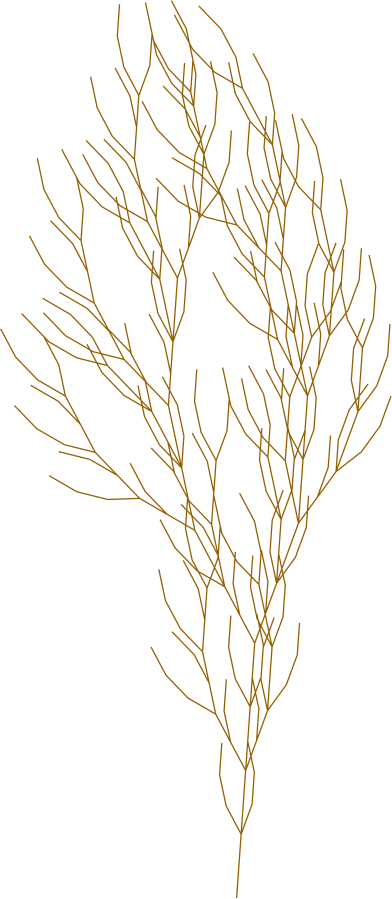
\includegraphics[height=7cm]{L-system-fractal.svg.png}
	\caption{Przykład stworzonej struktury za pomocą L systemu}
    \label{fig:lsystreeexample}
\end{figure}

Na rysunku \ref{fig:lsystreeexample} jest przykład zastosowania L systemu dla stworzenia 
fraktalnej struktury, która wygląda jak drzewo.



\section{Struktura L systemu}

\section{Interpretacja ciągu znaków}

\chapter{Implementacja} 

\section{Wykorzystane narzędzia}

\subsection{Język i środowisko}

\subsection{Biblioteka Proctree}

\subsection{Biblioteka nlohmann Json}

\section{Schemat działania}

\subsection{Głowne klasy}

\subsection{Symulacja wzrostu}

\chapter{Testy i rezultaty}

\section{Wydajność}
\section{Porównanie z innymi rozwiązaniami}

\chapter{Podsumowanie}

\chapter{Bibliografia}

\end{document}